
\documentclass[conference]{IEEEtran}
\IEEEoverridecommandlockouts
% The preceding line is only needed to identify funding in the first footnote. If that is unneeded, please comment it out.
\usepackage{cite}
\usepackage{amsmath,amssymb,amsfonts}
\usepackage{algorithmic}
\usepackage{graphicx}
\usepackage{textcomp}
\usepackage{xcolor}
\def\BibTeX{{\rm B\kern-.05em{\sc i\kern-.025em b}\kern-.08em
    T\kern-.1667em\lower.7ex\hbox{E}\kern-.125emX}}
\begin{document}

\title{CENG435 Term Project Part 2
}

\author{\IEEEauthorblockN{Ahmet Kürşad Şaşmaz - e2237824}
\and
\IEEEauthorblockN{Ali Şen - e2264661}
}

\maketitle

\section{Introduction}
In this CENG435 Term Project, participants worked on an already designed network topology. Explanation of who did what is written in a table at the end of the report. The topology has 5 nodes and 3 of them are routers one of them is sender(source node) and another of them is receiver(destination). We implemented reliable data transfer protocol based on User Datagram Protocol which we implemented in Part 1. Furthermore, we experimented sending through only one router and sending through two router (multi homing).\\

\section{Problem}

The problem was handling the data loss in two different sending routines. For both experiments, links between every node were configured with variable loss percentage and constant (3ms) delay. We are expected to handle this loss, and be sure the actual data is sent from source to destination the same. Moreover, we are expected to use pipelining while sending packets. For experiment 1, there is no special specifications except above. However, for experiment 2, we are expected to send and receive packets from which are/is connected to s of r1 and r2. Because, links between s-r1 and s-r2 may be down randomly. We have to handle this randomization and reset the topology according to alive links. Making easy to understand and use, we should implement generic code. To itemize, we are expected to:
\begin{itemize}
    \item Handle packet loss
    \item Send packets with pipelining
    \item Be sure every packet received without corruption
    \item Be sure all the data transmitted correctly
    \item Set a structure that downs link randomly
    \item Be aware of which link is alive and which is not
    \item Reset the topology according to alive links
    \item Split the data and send through alive links (i.e. multihoming)
\end{itemize}

\section{Solution and Methodology}

\subsection{Reliable Data Transfer Designs}

There are two possible choices for reliable data transfer. One of them is selective repeat and the other one is go-back-n. Since we are using the pipeline to send data consecutive we need a window size when the first sent packet acknowledge comes the base (so as the whole window) of the window will move to the next packet. In addition to this, the source node needs to has a timer for all packets sent to the destination node d. When the packets acknowledge does not come in the specific time we know that there is packet loss or the acknowledge of the packet exposed to delay.

\subsection{Selective Repeat}

The destination node has a buffer and uses the buffer when the expected packet number does not come. For instance, when the window size is 20 initially the expected packet number is 0 and when packet 0 loss the buffer keeps the other packets as [1,2,3,4 ,...,19] and when the source node can't take the acknowledge of the first packet it sent s node will send it again and if this time the packet reaches the destination, destination node d will take it and take the other packets from its buffer until the buffer is empty.

\subsection{Go-back-N}

Go-back-N is another pipelining implementation. Packets are sent as window size without waiting for the acknowledge of them. And if there is a packet loss source node s will send the whole window size from the packet number that lost. In this method, there is no buffer in destination node d and if there is a duplicate in the destination node d since the acknowledges of the packet can be lost source node s will assume that the packet couldn't reach the destination. \\
We choose go-back-n in our implementation. To use the time for the sent packet we import the time library of the python programming language. \\

To check the corruption of packets, we calculated checksums of every packet via md5 function. Then, we compared expected checksums and checksums that is in the packet to be ensured that the packet wasn't corrupted. For the only experiment 2, we define a thread that downs r1 and r2 link randomly. \\

To generalize the scripts, we write the common codes of scripts of nodes to a library script. Moreover, to reduce the workload while sending files to the nodes, configuring the nodes, executing the scripts on the nodes and getting the results of experiments, we implemented shell scripts that are run in local. Furthermore, all the experiment time data is stored by sender node (source s) relatively, we didn't need to synchronize the time between the nodes.

\section{Set Up The Environment}
\subsection{Network Topology}
There was 5 nodes on the topology. Names of the nodes were \textbf{s},\textbf{r1},\textbf{r2},\textbf{r3},\textbf{d}.
Connection link table is given below.
\begin{table}[ht]
\centering
\begin{tabular}{|l|l|}
\hline
\textbf{s}  & \textbf{r1} \\ \hline
\textbf{s}  & \textbf{r2} \\ \hline
\textbf{s}  & \textbf{r3} \\ \hline
\textbf{d}  & \textbf{r1} \\ \hline
\textbf{d}  & \textbf{r2} \\ \hline
\textbf{d}  & \textbf{r3} \\ \hline
\end{tabular}
\end{table}
As seen in the table the links between the routers are not used because they are not necessary for our experiments. That is why r1,r2 and r3 will behave like routers. S node will be the source node which will send the data and expect acknowledge of the packet if the packet has arrived to the destination node d. S node will take this information from the r3 node in Experiment 1 and r1 and r2 nodes in the experiment 2 since there is no direct connection between s and d nodes. Routers (r1,r2,r3) will only send the data they get from s node to d node when s sends data and d node to s node when d node sends the acknowledge of the packet to the s node.\\
\subsection{Configuration}

For every experiment there are three different loss percentages. We configure every node before doing the experiment with local shell scripts. In order that shell scripts in local work, ssh config file that is in the "~/.ssh" folder has to be configured with proper values. In all cases we have 3ms delay and we have configured packet loss percentages as 5\% 15\% and 38\% respectively. We applied these configurations to all nodes in the topology in a increasing packet loss percentage.Since delays are the same in 3 cases we did not update the delay.\\


\subsection{Server/Client Files}

Every node had capability to behave server and client at the same time. In order to provide this, threading paradigm was used. Every node had different purposes.S node read the input file which is 5 megabytes binary file and parse the file into a specific length of bytes.\\

We assign the byte length to a variable so that we can change it to see program behaviour. We compared the performance of the transmission. We see that when the byte length is less the transmission performance increases. However, we know that in the real world the more we increase the number of packets which we did by decreasing the size of packet the more loss or delay happens due to the noise and delays.S node also expects acknowledges of every packet it sends and if the acknowledges of the packet s node sends does not comes, s node sends it again. Moreover, s node computes the checksum of the packet and sends it to the destination node d to check if the packet is corrupted. Actually packets will never get corrupted since we did not configure it.\\

The destination node d listens r3 node to receive the packets from source node s. When d node gets the packet it control its checksum with the one d node calculated to see if the packet corrupted and sends the acknowledge to the source node s. In both experiments the destination node d behaves the same. It sends the acknowledges to the router (r1 or r2 or r3) which d node received the packet. \\

To provide 95\% confidence interval, we have to take more samples. However, because 5.000.000 bytes file size is too big, we set file size as 50.000 bytes and increased experiment repeat number. So, code implementation is set according to 50.000 bytes file size. If you want to increase or decrease it, please change global variable \textbf{totalLength} in \textbf{packet.py} \\


In the following section the topology nodes are explained clearly.\\ \\

\subsubsection{\textbf{s.py (s)}} 
\begin{itemize} 
    \item Read the input file \\
    
    \item Divide the data into files and store in a buffer \\
    
    \item Prepare packets with calculating checksum, adding send time , assigning sequence number for every part of data \\
    
    \item Send packets to the router(s) that is/are relative with the experiment \\
    
    \item Listen acknowledge packets from the router(s) that is/are relative with the experiment \\
    
    \item Check timeout for packets and do timeout routine \\
    
    \item For only experiment 2, down the links between s and (r1/r2) randomly\\ \\
\end{itemize}

\subsubsection{\textbf{r.py (r1-r2-r3)}}
\begin{itemize}
    \item Get data from source s and send it to destination d \\
    
    \item Get data from destination d and send it to source s\\ \\
\end{itemize}

\subsubsection{\textbf{d.py (d)}}
\begin{itemize}
    \item Listen the router(s) that is/are relative with the experiment \\
    
    \item If the packet has expected sequence number, write it to the output file \\
    
    \item Else just send the acknowledge packet of it\\ \\
\end{itemize}

\subsubsection{\textbf{packet.py}}
\begin{itemize}
    \item Pack a packet\\
    
    \item Unpack a packet\\
    
    \item Store global variables that are related with packets (packet length etc.)\\ \\
\end{itemize}

\subsubsection{\textbf{ipTable.py}}
\begin{itemize}
    \item Store IPs and ports as tuples in a dictionary with keywords in formatted as "x listens y" \\ \\
    
\end{itemize}

\subsubsection{\textbf{gen.py}}
\begin{itemize}
    \item Make related socket connections that is related according to the node that gen.py run in \\
    
    \item Close defined socket connections \\ \\
\end{itemize}

\subsection{Sending Files}

There is an already implemented shell script code that is run in local.\\
(\textbf{configureLinks.sh}) \\
\textbf{chmod +x sendingFiles.sh} \\
\textbf{./sendFiles.sh [s \textbar r1 \textbar r2 \textbar r3 \textbar d \textbar all]} \\ \\

\subsection{Configure The Nodes}

There is an already implemented shell script code that is run in local. (\textbf{configureLinks.sh}) \\
\textbf{chmod +x configureLinks.sh} \\
\textbf{./configureLinks.sh [experimentNumber] [configurationNumber]} \\

For experiment 1 : experimentNumber = 1 \\
For experiment 2 : experimentNumber = 2 \\

For 5\% loss percentage : configurationNumber = 1 \\
For 15\% loss percentage : configurationNumber = 2 \\
For 38\% loss percentage : configurationNumber = 3 \\

\subsection{To Up A Node}

There is an already implemented shell script code that is run in local. (\textbf{up.sh}) \\
\textbf{chmod +x up.sh} \\
To up a router \\
\textbf{./up.sh [\textbar r1 \textbar r2 \textbar r3]} \\ \\
To up source s \\
\textbf{./up.sh s [experimentNumber] [configurationNumber] [experimentTimes]} \\ \\
To up destination d \\
\textbf{./up.sh d [experimentNumber] [experimentTimes] } \\

For experiment 1 : experimentNumber = 1 \\
For experiment 2 : experimentNumber = 2 \\

For 5\% loss percentage : configurationNumber = 1 \\
For 15\% loss percentage : configurationNumber = 2 \\
For 38\% loss percentage : configurationNumber = 3 \\

\subsection{To Down A Node}

There is an already implemented shell script code that is run in local. (\textbf{up.sh}) \\
\textbf{chmod +x down.sh} \\
\textbf{./down.sh [s \textbar r1 \textbar r2 \textbar r3 \textbar d \textbar experiment \textbar routers \textbar all]} \\ \\
For only down s and d use \textbf{experiment} \\
For only down routers use \textbf{routers} \\
For down all nodes use \textbf{all} \\ \\

\subsection{Getting Results}

There is an already implemented shell script code that is run in local. (\textbf{getResults.sh}) \\
\textbf{chmod +x getResults.sh} \\
\textbf{./getResults.sh} \\

This shell script copies results.txt file from node s to local as \textbf{filledResults.txt} \\ \\ 

\section{Experiments}

\subsection{General Information About Experiments}

For the both experiments the similar methodologies are used. Generally, while performing our experiment firstly we executed the Configurelinks.sh script with the correct parameters that will perform the correct experiment. By saying correct parameters, there are two consecutive numbers that will adjust the all nodes accordingly the experiment we want to perform. Our parameter form is like this: \\
\begin{table}[ht]
\begin{tabular}{|l|l|l|}
\hline
Parameter 1 & Parameter 2 & Experiment Performed                          \\ \hline
1           & 1           & Experiment 1 with loss value of 5\%  \\ \hline
1           & 2           & Experiment 1 with loss value of 15\% \\ \hline
1           & 3           & Experiment 1 with loss value of 35\% \\ \hline
2           & 1           & Experiment 2 with loss value of 5\%  \\ \hline
2           & 2           & Experiment 2 with loss value of 15\% \\ \hline
2           & 3           & Experiment 2 with loss value of 35\% \\ \hline
\end{tabular}
\end{table} \\ 

After applying the configuration we want, then we will first execute the d.py in the d node and r.py in the nodes r1, r2 and r3 according to the the experiment number. For experiment 1, it is enough to execute this script in the r3 node, for experiment 2 we will execute it in the both r1, r2 nodes.

\subsection{Experiment 1}

\begin{figure}[h]
  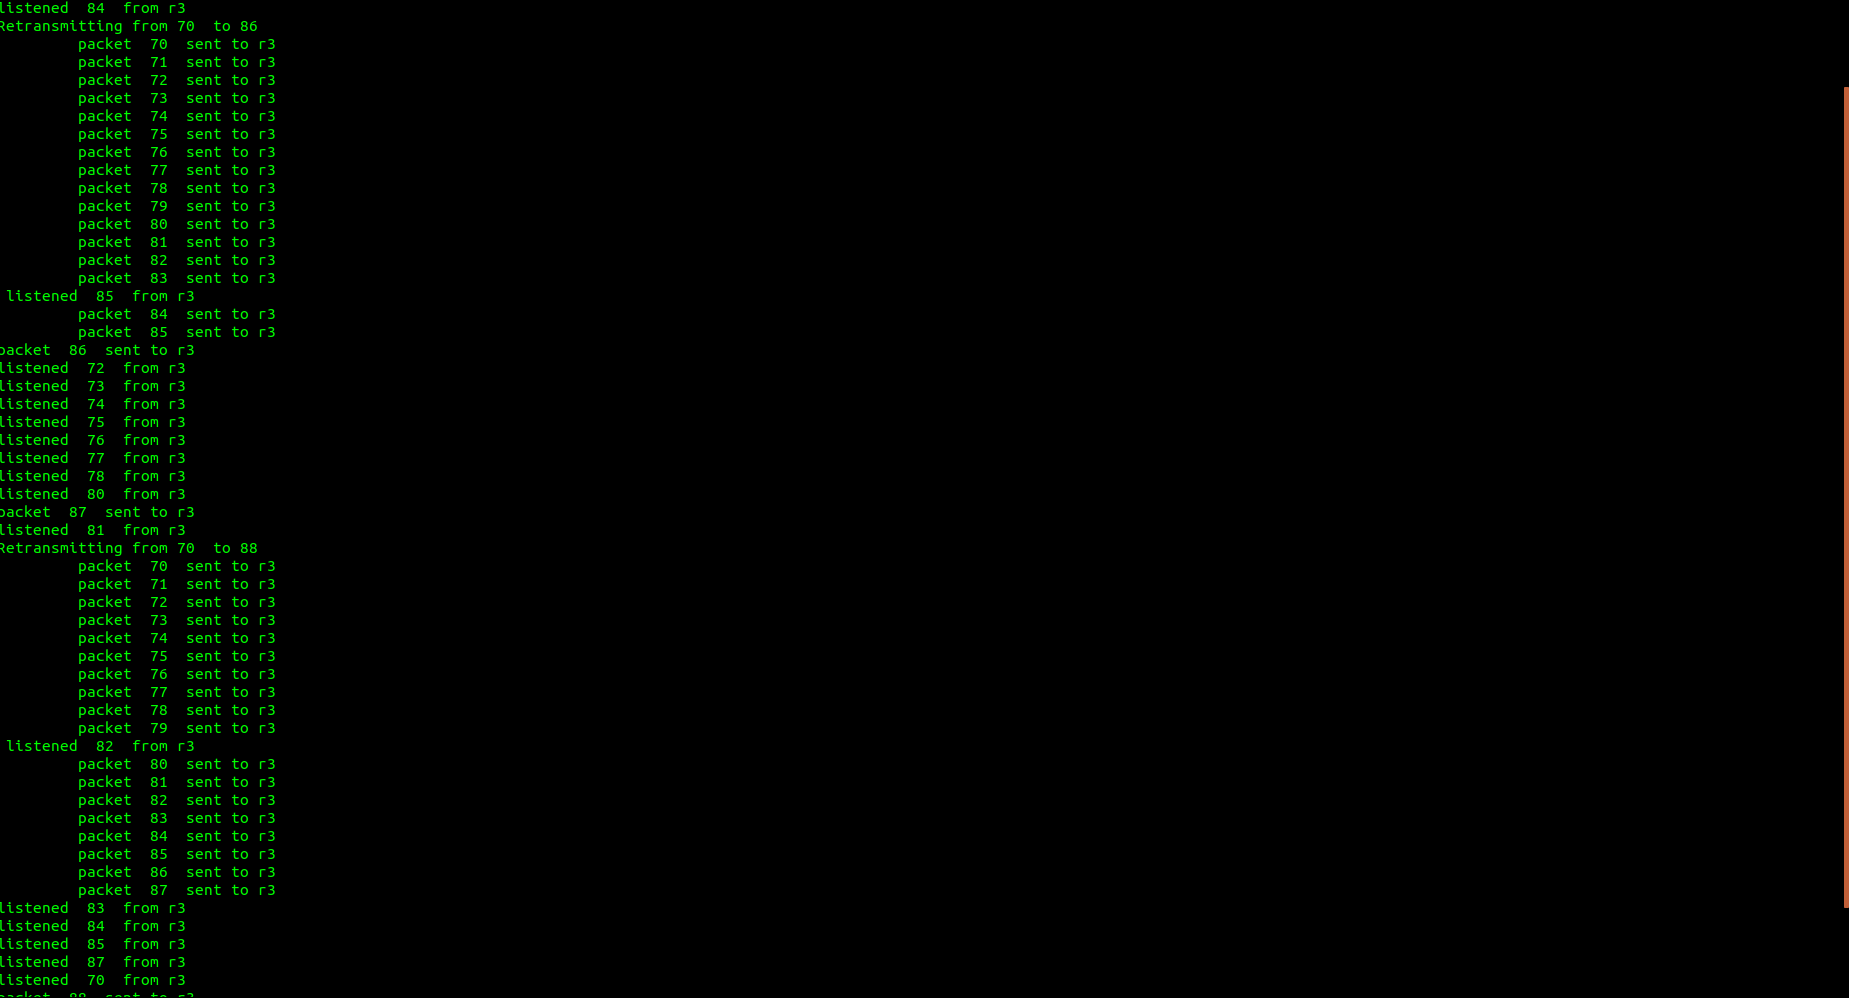
\includegraphics[width=\linewidth]{experiment1.png}
  \caption{Screenshot while experiment 1 is running.}
  \label{fig:ss1}
\end{figure}

Figure \ref{fig:ss1} Screenshot while experiment 1 is running.

When a packet exposed to a loss, this is known by the source node s by the timeout of the packet. That means the acknowledge of the packet does not come in the expected time and the s node sends the data again as we explained in the go-back-n section.

\subsection{Experiment 2}

\begin{figure}[h]
  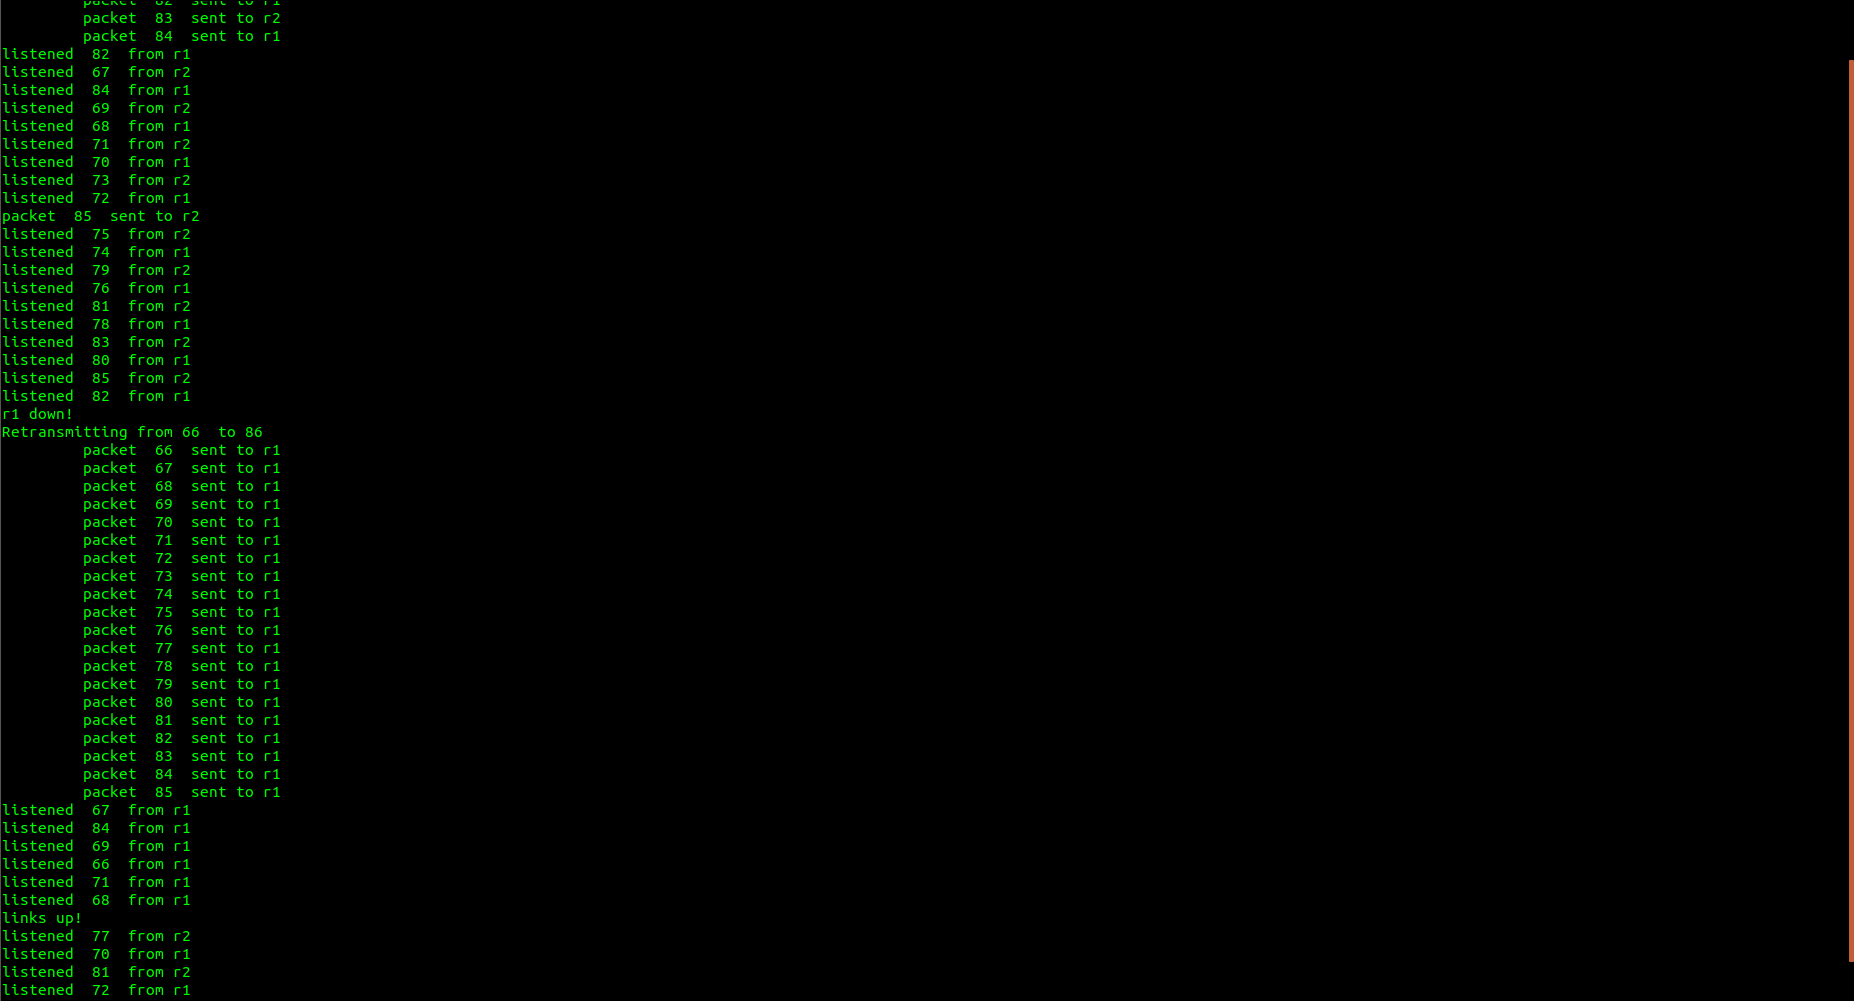
\includegraphics[width=\linewidth]{experiment2.png}
  \caption{Screenshot while experiment 2 is running.}
  \label{fig:ss2}
\end{figure}

Figure \ref{fig:ss2} Screenshot while experiment 2 is running.

When a packet exposed to a loss, this is known by the source node s by the timeout of the packet. The node uses go-back-n. In addition to this, links between s and r1/r2 are randomly down. Our implementation knows which connection is on which is not. If a link is down, the node continues to send packets through open connection. If both of the links are online, the script take modula of current sequence number, prepare packet and send it through proper socket connections.

\subsection{Results}

\begin{figure}[h]
  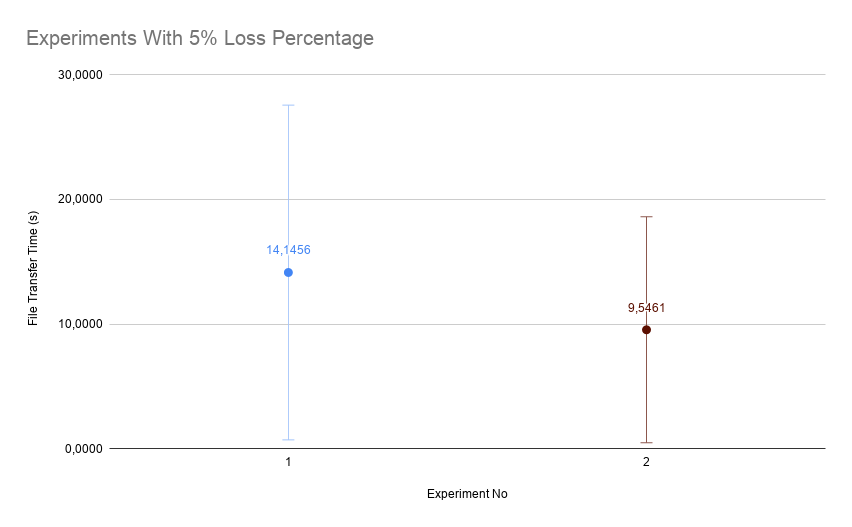
\includegraphics[width=\linewidth]{experimentPlot.png}
  \caption{File Transfer Times With Respect To Experiments with 5\% Loss Percentage}
  \label{fig:plot}
\end{figure}

Figure \ref{fig:plot} File Transfer Times With Respect To Experiments with 5\% Loss Percentage

\begin{table}[h]
\centering
\begin{tabular}{|l|l|l|l|}
\hline
Experiment Number & $\mu$ & $\sigma$ & Error \\ \hline
1 & 14.1456s  & 68.5623s     & 13.4383s     \\ \hline
2 & 9.5461s & 46.2689s     & 9.0687s     \\ \hline
\end{tabular}
\end{table}

X axis shows experiment number, Y axis show file transfer time in terms of seconds. In experiment 1, data sent through router r3. In experiment 2, data were splitted and sent through router r1 and r2 at the same time. As shown in the plot graph and data table, we can say that, sending packets through more than one router at the same time, decrease file transfer time. We have a hypothesis that file transfer time proportional to file size divided by number of routers that is used.

\section{Discussions}

The advantage of packet switching is sending and receiving data at the same time when the link is being used. But on the other hand, we observe some packet loss which we didn't want in real life and that is the disadvantage of such a topology. In fact in our topology we will not have any loss or delay if we did not configure the nodes. However, to experience the real world problems we need to configure the nodes.\\

Unlike our topology actual routers are also connected each other. The reason for this is to prevent of packet loss or send packet faster by sending the data to the other routers which have less data to sent in its buffer. \\

We see that in the second experiment packet delivery is faster than the first experiment. That is the advantage of multihoming when we use 2 routers to transmit a file it is much faster even if we use the shortest path in the first experiment. \\

To handle packet loss, send the file not corrupted, our implementation got deeper calculations and methods. By deeper, we had to think every possibility that packet can be in. \\

In real life, due to connection lost and noise, packet may be lost or corrupted. To be ensure that data is received by destination, we have to implement some methods that guarantee packet are sent and notify the sender.

\section{Who Did What}
\begin{table}[h]
\centering
\begin{tabular}{|l|l|}
\hline
Ali Şen & Ahmet Kürşad Şaşmaz \\ \hline
\begin{minipage}[h]{0.2\textwidth}
    \begin{itemize}
    \item Introduction of The Report
    \item Packet Library
    \item Script of Receiver Node (Destination)
    \item Configuration Script Files
    \item Solution and Methodology Part of The Report
    \item Experiments Part of The Report
    \end{itemize}
  \end{minipage}
&
\begin{minipage}[h]{0.2\textwidth}
    \begin{itemize}
    \item Set Up The Environment Part of The Report
    \item Script of Common Codes of Scripts
    \item Script of Sender Node (Source)
    \item Local Script Files
    \item ReadMe File
    \item Problem Part of The Report
    \item Discussion Part of The Report
    \end{itemize}
  \end{minipage}
\\ \hline
\end{tabular}
\end{table}

\end{document}
